\documentclass{beamer}
\usetheme{Madrid}
\usecolortheme{default}

% Packages
\usepackage{amsmath}
\usepackage{amsfonts}
\usepackage{amsthm}
\usepackage{amssymb}
\usepackage{mathrsfs}
\usepackage{mathtools}
\usepackage{bbm}
\usepackage{bm}
\usepackage{tikz}
\usepackage{graphicx}
\usepackage[authoryear]{natbib}

% Math shortcuts from main.tex
\newcommand{\E}{\mathbb{E}}
\newcommand{\Var}{\mathrm{Var}}
\newcommand{\Cov}{\mathrm{Cov}}
\newcommand{\bbm}[1]{\mathbbm{#1}}
\newcommand{\bb}[1]{\mathbb{#1}}
\newcommand{\indicator}{\mathbbm{1}}
\newcommand{\de}{\textsc{de}}
\newcommand{\bie}{\textsc{bie}}
\newcommand{\wie}{\textsc{wie}}
\newcommand{\horthom}{\textup{ht}}
\newcommand{\haj}{\textup{haj}}
\newcommand{\pscore}[1]{\pi_{#1}}
\newcommand{\pr}{\textup{pr}}
\newcommand{\sumi}{\sum_{i=1}^n}
\newcommand{\sumj}{\sum_{j=1}^n}
\newcommand{\sumk}{\sum_{k=1}^m}
\newcommand{\bY}{\boldsymbol{Y}}
\newcommand{\bA}{\boldsymbol{A}}
\newcommand{\bZ}{\boldsymbol{Z}}
\newcommand{\cN}{\mathcal{N}}
\newcommand{\cG}{\mathcal{G}}
\newcommand{\bOmega}{\boldsymbol{\Omega}}
\newcommand{\bGamma}{\boldsymbol{\Gamma}}

\title[Within-cluster and Between-cluster Spillover Effects]{Estimating within-cluster and between-cluster spillover effects in randomized saturation designs}

\author[Lu, Shi, Ding]{
Sizhu Lu\inst{1} \and 
Lei Shi\inst{2} \and 
Peng Ding\inst{1}
}

\institute[UC Berkeley]{
\inst{1} Department of Statistics, University of California, Berkeley \\
\inst{2} Division of Biostatistics, University of California, Berkeley
}

\date{\today}

\begin{document}

\frame{\titlepage}

\begin{frame}
\frametitle{Outline}
\tableofcontents
\end{frame}

\section{Introduction}

\begin{frame}
\frametitle{Motivation}
\begin{itemize}
\item Randomized saturation designs are widely used to study causal effects with network interference
\item Most existing studies focus on within-cluster interference
\item Assume away between-cluster spillover effects
\item Often unrealistic in practice!
\end{itemize}

\vspace{0.5cm}
\textbf{Leading Example:} Cash transfer program in rural Kenya \citep{egger2022general}
\begin{itemize}
\item Villages may interact across sublocations (clusters)
\item Geographic proximity creates spillover effects
\end{itemize}
\end{frame}

\begin{frame}
\frametitle{Kenya Cash Transfer Study}
\textbf{Two-stage design:}
\begin{enumerate}
\item Sublocations randomly assigned to high/low saturation
\item Within sublocations: villages randomly assigned to treatment
\end{enumerate}

\vspace{0.5cm}
\textbf{Two sources of interference:}
\begin{itemize}
\item \textbf{Within-sublocation:} villages in same sublocation affect each other
\item \textbf{Between-sublocation:} geographically close villages in different sublocations
\end{itemize}

\vspace{0.5cm}
\begin{center}
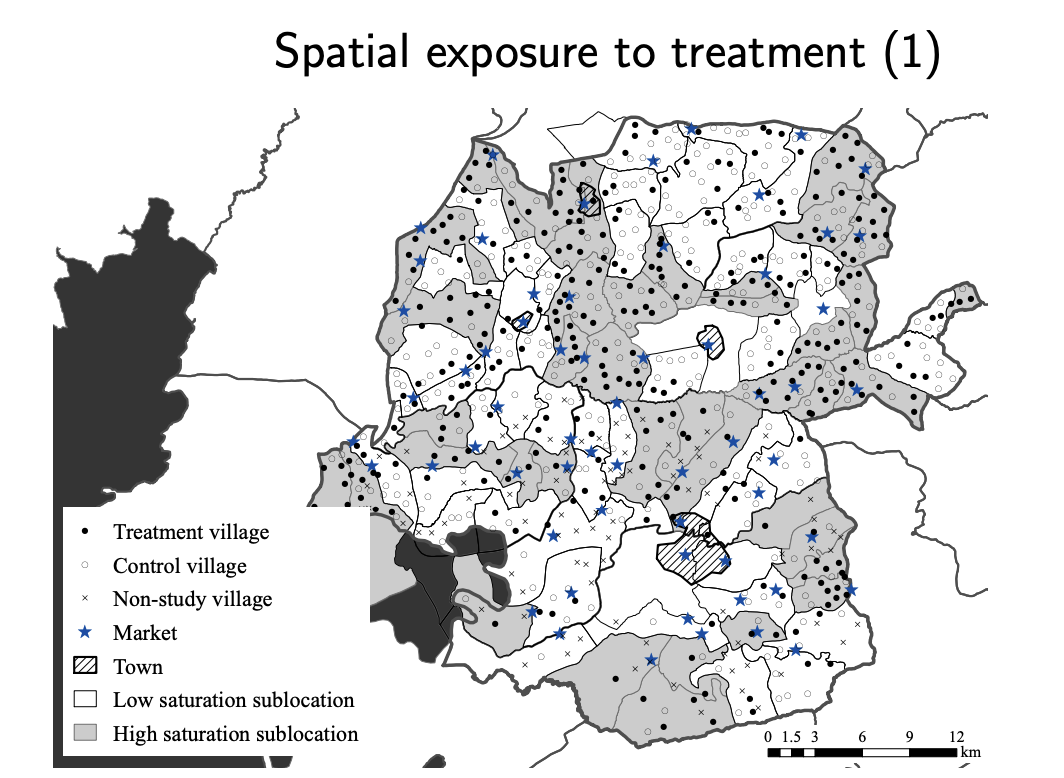
\includegraphics[width=0.6\textwidth]{spatial.png}
\end{center}
\end{frame}

\section{Framework}

\begin{frame}
\frametitle{Setup and Notation}
\begin{itemize}
\item $n$ villages indexed by $i = 1, \ldots, n$
\item $k(i)$: sublocation containing village $i$
\item $\cG_{+i}$: set of villages geographically close to village $i$
\item $A_i \in \{0,1\}$: treatment assignment for village $i$
\end{itemize}

\vspace{0.5cm}
\textbf{Exposure mapping:} $d_i(\bA) = (A_i, S_i, H_i)$ where
\begin{align}
S_i &= \indicator\left\{\frac{\sum_{j\neq i}\indicator\{k(j)=k(i)\} A_j}{\sum_{j\neq i}\indicator\{k(j)=k(i)\}} > \frac{1}{2}\right\} \\
H_i &= \indicator\left\{\frac{\sum_j \indicator\{k(j)\neq k(i), j\in\cG_{+i}\}A_j}{\sum_j \indicator\{k(j)\neq k(i), j\in\cG_{+i}\}} > \frac{1}{2}\right\}
\end{align}
\end{frame}

\begin{frame}
\frametitle{Potential Outcomes}
\begin{itemize}
\item $Y_i(a,s,h)$: potential outcome for village $i$ under exposure $(a,s,h)$
\item $a$: own treatment status
\item $s$: within-cluster exposure (majority treated in same sublocation)
\item $h$: between-cluster exposure (majority treated among connected villages in other sublocations)
\end{itemize}

\vspace{0.5cm}
\textbf{Key assumption:} No interference beyond this exposure mapping
$$Y_i = Y_i(A_i, S_i, H_i)$$
\end{frame}

\section{Causal Parameters}

\begin{frame}
\frametitle{Direct Effect}
\textbf{Controlled direct effect:}
$$\de(s,h) = n^{-1}\sumi Y_i(1,s,h) - n^{-1}\sumi Y_i(0,s,h)$$

\vspace{0.5cm}
\textbf{Marginal direct effect:}
$$\de = n^{-1}\sumi E_{\bA_{(-i)}}\{Y_i(1,S_i,H_i)\} - n^{-1}\sumi E_{\bA_{(-i)}}\{Y_i(0,S_i,H_i)\}$$

\vspace{0.5cm}
\begin{itemize}
\item $\de(s,h)$: effect of treatment holding spillover exposures fixed
\item $\de$: effect marginalizing over spillover distribution
\item $\de$ depends on treatment assignment mechanism
\end{itemize}
\end{frame}

\begin{frame}
\frametitle{Within-Cluster Indirect Effects}
\textbf{Controlled within-cluster indirect effect:}
$$\wie(s,s',h) = n^{-1}\sumi Y_i(0,s,h) - n^{-1}\sumi Y_i(0,s',h)$$

\vspace{0.5cm}
\textbf{Marginal within-cluster indirect effect:}
$$\wie(s,s') = n^{-1}\sumi E_{\bA_{(-i)}|S_i=s}\{Y_i(0,s,H_i)\} - n^{-1}\sumi E_{\bA_{(-i)}|S_i=s'}\{Y_i(0,s',H_i)\}$$

\vspace{0.5cm}
\begin{itemize}
\item Effect of changing within-cluster treatment saturation
\item Holding own treatment at 0 and between-cluster exposure fixed (controlled) or marginalized (marginal)
\end{itemize}
\end{frame}

\begin{frame}
\frametitle{Between-Cluster Indirect Effects}
\textbf{Controlled between-cluster indirect effect:}
$$\bie(s,h,h') = n^{-1}\sumi Y_i(0,s,h) - n^{-1}\sumi Y_i(0,s,h')$$

\vspace{0.5cm}
\textbf{Marginal between-cluster indirect effect:}
$$\bie(h,h') = n^{-1}\sumi E_{\bA_{(-i)}|H_i=h}\{Y_i(0,S_i,h)\} - n^{-1}\sumi E_{\bA_{(-i)}|H_i=h'}\{Y_i(0,S_i,h')\}$$

\vspace{0.5cm}
\begin{itemize}
\item Effect of changing between-cluster treatment exposure
\item Novel contribution: first to formalize between-cluster spillovers in randomized saturation designs
\end{itemize}
\end{frame}

\begin{frame}
\frametitle{Policy-Specific Parameters}
For treatment assignment policy $\psi$:

\begin{align}
\de_\psi &= n^{-1}\sumi E_\psi\{Y_i(1,S_i,H_i)\} - n^{-1}\sumi E_\psi\{Y_i(0,S_i,H_i)\} \\
\wie_\psi &= n^{-1}\sumi E_\psi\{Y_i(0,1,H_i)\} - n^{-1}\sumi E_\psi\{Y_i(0,0,H_i)\} \\
\bie_\psi &= n^{-1}\sumi E_\psi\{Y_i(0,S_i,1)\} - n^{-1}\sumi E_\psi\{Y_i(0,S_i,0)\}
\end{align}

\vspace{0.5cm}
Can compare policies $\psi_1$ vs $\psi_2$ via:
$$\de_{\psi_1} - \de_{\psi_2}, \quad \wie_{\psi_1} - \wie_{\psi_2}, \quad \bie_{\psi_1} - \bie_{\psi_2}$$
\end{frame}

\section{Estimation}

\begin{frame}
\frametitle{Estimating Average Potential Outcomes}
Target: $\bar{Y}(a,s,h) = n^{-1}\sumi Y_i(a,s,h)$

\vspace{0.5cm}
\textbf{Horvitz-Thompson estimator:}
$$\hat{Y}^{\horthom}(a,s,h) = n^{-1}\sumi\frac{\indicator\{A_i=a, S_i=s, H_i=h\}}{\pscore{i}(a,s,h)}Y_i$$

\vspace{0.5cm}
\textbf{Hajek estimator:}
$$\hat{Y}^{\haj}(a,s,h) = \frac{n^{-1}\sumi\frac{\indicator\{A_i=a, S_i=s, H_i=h\}}{\pscore{i}(a,s,h)}Y_i}{n^{-1}\sumi\frac{\indicator\{A_i=a, S_i=s, H_i=h\}}{\pscore{i}(a,s,h)}}$$

where $\pscore{i}(a,s,h) = \pr(A_i=a, S_i=s, H_i=h)$
\end{frame}

\begin{frame}
\frametitle{Policy-Specific Estimation}
Use re-weighting with weights $\gamma_i(a,s,h)$:

$$\hat{Y}^{\horthom}(a,s,h;\Gamma) = n^{-1}\sumi\frac{\indicator\{A_i=a, S_i=s, H_i=h\}\gamma_i(a,s,h)}{\pscore{i}(a,s,h)}Y_i$$

\vspace{0.5cm}
For policy-specific effects, choose:
\begin{align}
\gamma_{i,\psi}^{\de}(a,s,h) &= \pscore{i,\psi}(\cdot,s,h) \\
\gamma_{i,\psi}^{\wie}(a,s,h) &= \pscore{i,\psi}(\cdot,\cdot,h) \\
\gamma_{i,\psi}^{\bie}(a,s,h) &= \pscore{i,\psi}(\cdot,s,\cdot)
\end{align}
\end{frame}

\begin{frame}
\frametitle{Effect Estimators}
\textbf{Controlled effects:}
\begin{align}
\hat{\de}^*(s,h) &= \hat{Y}^*(1,s,h) - \hat{Y}^*(0,s,h) \\
\hat{\wie}^*(s,s',h) &= \hat{Y}^*(0,s,h) - \hat{Y}^*(0,s',h) \\
\hat{\bie}^*(s,h,h') &= \hat{Y}^*(0,s,h) - \hat{Y}^*(0,s,h')
\end{align}

\vspace{0.5cm}
\textbf{Marginal effects:}
\begin{align}
\hat{\de}^* &= \hat{Y}^*(1) - \hat{Y}^*(0) \\
\hat{\wie}^*(s,s') &= \hat{Y}^*(0,s) - \hat{Y}^*(0,s') \\
\hat{\bie}^*(h,h') &= \hat{Y}^*(0,h) - \hat{Y}^*(0,h')
\end{align}

where $* \in \{\horthom, \haj\}$
\end{frame}

\section{Theoretical Properties}

\begin{frame}
\frametitle{Asymptotic Variance - Key Result}
For weighted Horvitz-Thompson estimator:
\begin{align}
&\text{Var}\{\hat{Y}^{\horthom}(a,s,h;\Gamma)\} \\
&= n^{-2}\sumi \frac{1-\pscore{i}(a,s,h)}{\pscore{i}(a,s,h)}\{\gamma_i(a,s,h)Y_i(a,s,h)\}^2 \\
&\quad + n^{-2}\sumi\sum_{j\neq i}\frac{\pscore{ij}(a,s,h;a,s,h) - \pscore{i}(a,s,h)\pscore{j}(a,s,h)}{\pscore{i}(a,s,h)\pscore{j}(a,s,h)} \\
&\qquad \times \gamma_i(a,s,h)\gamma_j(a,s,h)Y_i(a,s,h)Y_j(a,s,h)
\end{align}

\vspace{0.5cm}
Can be written compactly as:
$$\text{Var}\{\hat{Y}^{\horthom}(a,s,h;\Gamma)\} = n^{-2}\bY(a,s,h)^T\bGamma(a,s,h)\bOmega(a,s,h)\bGamma(a,s,h)\bY(a,s,h)$$
\end{frame}

\begin{frame}
\frametitle{Asymptotic Variance - Hajek Estimator}
For weighted Hajek estimator, define centered potential outcomes:
$$\tilde{Y}_i(a,s,h) = Y_i(a,s,h) - \frac{n^{-1}\sumi \gamma_i(a,s,h)Y_i(a,s,h)}{n^{-1}\sumi\gamma_i(a,s,h)}$$

\vspace{0.3cm}
Then:
\begin{align}
&\text{AVar}\{\hat{Y}^{\haj}(a,s,h;\Gamma)\} \\
&= n^{-2}\sumi \frac{1-\pscore{i}(a,s,h)}{\pscore{i}(a,s,h)}\{\gamma_i(a,s,h)\tilde{Y}_i(a,s,h)\}^2 \\
&\quad + n^{-2}\sumi\sum_{j\neq i}\frac{\pscore{ij}(a,s,h;a,s,h) - \pscore{i}(a,s,h)\pscore{j}(a,s,h)}{\pscore{i}(a,s,h)\pscore{j}(a,s,h)} \\
&\qquad \times \gamma_i(a,s,h)\gamma_j(a,s,h)\tilde{Y}_i(a,s,h)\tilde{Y}_j(a,s,h)
\end{align}

Compactly: $n^{-2}\tilde{\bY}(a,s,h)^T\bGamma(a,s,h)\bOmega(a,s,h)\bGamma(a,s,h)\tilde{\bY}(a,s,h)$
\end{frame}

\begin{frame}
\frametitle{Covariance Structure - Both Estimators}
\textbf{Horvitz-Thompson covariance:}
For $(a,s,h) \neq (a',s',h')$:
\begin{align}
&\text{Cov}\{\hat{Y}^{\horthom}(a,s,h;\Gamma), \hat{Y}^{\horthom}(a',s',h';\Gamma)\} \\
&= -n^{-2}\sumi \gamma_i(a,s,h)\gamma_i(a',s',h')Y_i(a,s,h)Y_i(a',s',h') \\
&\quad + n^{-2}\sumi\sum_{j\neq i}\frac{\pscore{ij}(a,s,h;a',s',h') - \pscore{i}(a,s,h)\pscore{j}(a',s',h')}{\pscore{i}(a,s,h)\pscore{j}(a',s',h')} \\
&\qquad \times \gamma_i(a,s,h)\gamma_j(a',s',h')Y_i(a,s,h)Y_j(a',s',h')
\end{align}

\textbf{Hajek covariance:} Same form but with $\tilde{Y}_i(a,s,h)$ and $\tilde{Y}_j(a',s',h')$
\end{frame}

\section{Regression Analysis}

\begin{frame}
\frametitle{Saturated Regression}
\textbf{Fully saturated regression:}
$$Y_i \sim \sum_{a,s,h} \indicator\{A_i=a, S_i=s, H_i=h\}$$

\vspace{0.5cm}
\textbf{Partially saturated regression:}
$$Y_i \sim 1 + A_i + \tilde{S}_i + \tilde{H}_i + A_i\tilde{S}_i + A_i\tilde{H}_i$$

where $\tilde{S}_i$ and $\tilde{H}_i$ are centered at population means

\vspace{0.5cm}
\begin{itemize}
\item Coefficient of $A_i$ estimates direct effect $\de$
\item Coefficients of $\tilde{S}_i, \tilde{H}_i$ estimate "overlap" versions of indirect effects
\item More efficient than IPW when model is correctly specified
\end{itemize}
\end{frame}

\begin{frame}
\frametitle{Overlap Indirect Effects}
From centered regression, we recover:

\begin{align}
\wie^{\text{o}} &= \frac{n^{-1}\sumi \pi_{S,i}(1-\pi_{S,i})E\{Y_i(0,1,H_i)-Y_i(0,0,H_i)\}}{n^{-1}\sumi \pi_{S,i}(1-\pi_{S,i})} \\
\bie^{\text{o}} &= \frac{n^{-1}\sumi \pi_{H,i}(1-\pi_{H,i})E\{Y_i(0,S_i,1)-Y_i(0,S_i,0)\}}{n^{-1}\sumi \pi_{H,i}(1-\pi_{H,i})}
\end{align}

\vspace{0.5cm}
\begin{itemize}
\item $\pi_{S,i}, \pi_{H,i}$: population probabilities of spillover exposure
\item Weighted averages of unit-level indirect effects
\item Different from our main estimands but still policy-relevant
\end{itemize}
\end{frame}

\section{Application}

\begin{frame}
\frametitle{Application to Kenya Study}
\textbf{Plans for empirical analysis:}
\begin{enumerate}
\item Re-analyze \cite{egger2022general} data with our framework
\item Estimate within-cluster and between-cluster spillover effects
\item Compare with original results that ignored between-cluster spillovers
\item Assess policy implications of accounting for geographic spillovers
\end{enumerate}

\vspace{0.5cm}
\textbf{Expected contributions:}
\begin{itemize}
\item Quantify magnitude of between-cluster spillovers
\item Show importance of accounting for geographic proximity
\item Demonstrate practical relevance of our methodology
\end{itemize}
\end{frame}

\section{Discussion}

\begin{frame}
\frametitle{Main Contributions}
\begin{enumerate}
\item \textbf{Novel framework:} First to formalize both within- and between-cluster spillovers in randomized saturation designs

\item \textbf{Causal identification:} Clear definitions of direct and indirect effects under complex interference

\item \textbf{Statistical theory:} Rigorous asymptotic theory for IPW and regression estimators

\item \textbf{Practical relevance:} Framework applies to many real experiments with geographic spillovers
\end{enumerate}
\end{frame}

\begin{frame}
\frametitle{Future Directions}
\begin{enumerate}
\item \textbf{Model-assisted approaches:} Incorporate outcome models for efficiency gains

\item \textbf{Continuous exposures:} Extend beyond binary spillover indicators

\item \textbf{Multiple networks:} Handle multiple types of connections simultaneously

\item \textbf{Optimal design:} Design randomization to maximize power for spillover detection

\item \textbf{Robustness:} Study sensitivity to exposure mapping specification
\end{enumerate}
\end{frame}

\begin{frame}
\frametitle{Practical Considerations}
\textbf{Implementation challenges:}
\begin{itemize}
\item Defining geographic neighborhoods $\cG_{+i}$
\item Handling isolated units with no cross-cluster neighbors
\item Ensuring sufficient overlap for identification
\item Computational complexity with large networks
\end{itemize}

\vspace{0.5cm}
\textbf{Solutions:}
\begin{itemize}
\item Use distance-based or k-nearest neighbor definitions
\item Set $H_i = 0$ for isolated units (with variance adjustments)
\item Check overlap conditions in design phase
\item Leverage sparsity in network structures
\end{itemize}
\end{frame}

\begin{frame}
\frametitle{Conclusion}
\begin{itemize}
\item Randomized saturation designs can have complex spillover structures
\item Ignoring between-cluster spillovers may lead to biased inference
\item Our framework provides tools to estimate and test for these effects
\item Rigorous statistical theory supports practical implementation
\item Application to real data will demonstrate empirical relevance
\end{itemize}

\vspace{0.5cm}
\begin{center}
\textbf{Thank you!}
\end{center}
\end{frame}

\begin{frame}[allowframebreaks]
\frametitle{References}
\bibliographystyle{apalike}
\bibliography{ref}
\end{frame}

\end{document}
